A interação entre o ser humano e sua realidade tecnológica tem sido um tema de reflexão constante. Martin Heidegger, em "O Ser e o Tempo", propõe que nossa relação profunda com a tecnologia impacta de maneira determinante a qualidade de nossa experiência existencial \cite{2012_Silva_DISSERTATION}. Observando o gesto quase instintivo de deslizar sobre uma tela sensível ao toque, é possível evidenciar esta perspectiva heideggeriana: à medida que dominamos tal interface, a fronteira entre humano e digital se torna menos perceptível, integrando nossa experiência no mundo digital de maneira mais orgânica.

Complementarmente, o filósofo Merleau-Ponty, em sua análise fenomenológica do corpo, ressalta a centralidade do corpo como mediador em nossa relação com o mundo \cite{2011_MerleauPonty_BOOK}. Dispositivos digitais contemporâneos, além de serem ferramentas, tornam-se extensões corpóreas, afetando diretamente como percebemos e nos conectamos com a realidade. Merleau-Ponty já destacava a maneira como objetos externos, como um chapéu, podem ser incorporados à nossa percepção corporal.

Esta compreensão fenomenológica encontra ecos em descobertas recentes nos campos da neurofisiologia e neuropsicologia. Por exemplo, o estudo de \citeonline{2004_Maravita} evidencia que o uso de ferramentas modifica a representação neural do corpo em macacos, integrando-as ao 'esquema corporal'. Esse fenômeno sugere uma adaptação cerebral à extensão sensorial proporcionada pela ferramenta, reforçando a ideia de que dispositivos como smartphones reconfiguram nosso esquema corporal. Esta relação entre corpo, ferramentas e tecnologia é ilustrada na \autoref{fig:corpo_tecnologia}. Ao usar a câmera de um smartphone, nosso cérebro não só reconhece o dispositivo como uma ferramenta útil, mas também o integra como uma extensão dos nossos olhos, ampliando nossa capacidade de perceber e capturar o mundo.

\begin{figure}[ht]
	\centering
	\begin{subfigure}{0.45\textwidth}
		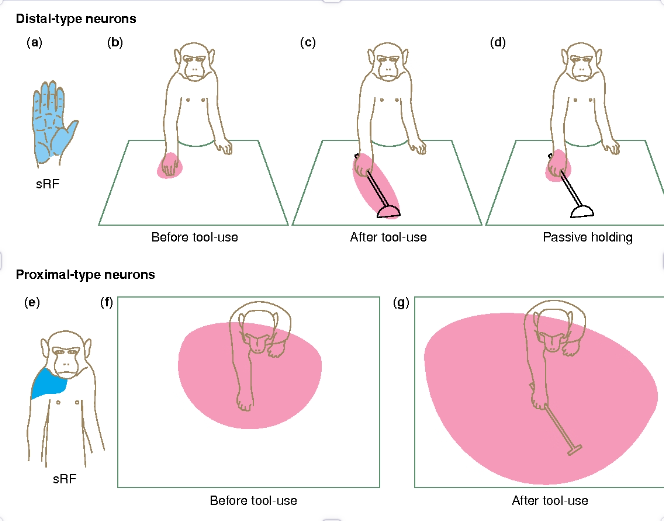
\includegraphics[width=\linewidth]{images/tools_for_the_body.png}
        \caption*{\citeonline{2004_Maravita}}
	\end{subfigure}
	\hfill
	\begin{subfigure}{0.45\textwidth}
		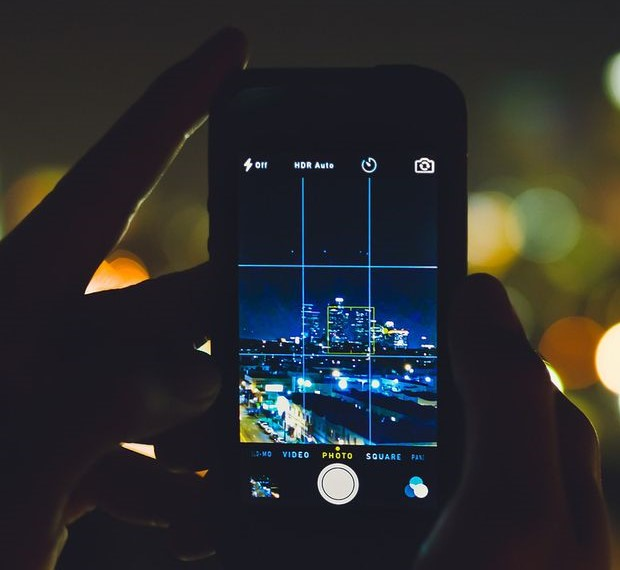
\includegraphics[width=\linewidth]{images/tools_for_the_mind.jpg}
		\caption*{Free-Photos/Pixabay}
	\end{subfigure}
	\caption{Representações da interconexão entre corpo e tecnologia: (Esquerda) Adaptação neural em macacos ao uso de ferramentas, exemplificando a extensão corpórea. (Direita) A interação humana com a tecnologia digital, simbolizada pelo uso de um smartphone.}
	\label{fig:corpo_tecnologia}
\end{figure}

Ao considerarmos uma intersecção entre as ideias de Heidegger e o estudo contemporâneo dessas ferramentas tecnológicas, percebemos a relevância do conceito de \textit{Zuhandenheit} ou tecnificação das mãos, que descreve como as ferramentas se integram em nossas atividades cotidianas de forma fluida e transparente. No entanto, essa tecnificação excessiva pode levar à inautenticidade e à perda de uma conexão genuína com nosso ser.

Em uma dimensão mais contemporânea, Pierre Lévy, em suas reflexões sobre o ciberespaço, destaca como a virtualização e a conectividade digital transformam a inteligência coletiva e a experiência social \cite{2010_Levy_BOOK}. O smartphone, neste contexto, não é apenas uma extensão do corpo, mas um portal para um espaço onde os indivíduos coletivamente constroem conhecimento e significado. Contudo, esse entrelaçamento íntimo com a tecnologia traz consigo dilemas. Jacques Derrida introduz o conceito de \textit{hauntologia}, que pode contextualizar o sentimento crescente de alienação no ciberespaço. Esse conceito se refere à presença dos "fantasmas" ou promessas do passado que continuam a assombrar o presente. 

O entusiasmo da virada do milênio, representado por shoppings centers e a bolha \textit{dotcom} da década de 1990, sugeria infinitas possibilidades de conexão e prosperidade. No entanto, hoje, muitos desses shoppings estão vazios e abandonados, assim como muito do ciberespaço da web 1.0, como IRCs, fóruns, páginas MySpace, Fotolog, Flogão, etc. Esses espaços abandonados foram ressignificados como parte de uma estética kitsch e gótica, lembrados principalmente em subculturas como o \textit{Vaporwave} e em seriados como \textit{Stranger Things}. A nova web 2.0 no seu maior exemplo de \textit{hauntologia} prometia ser uma rede social, mas o que vivemos hoje é uma realidade efêmera, em constante mudança e faminta por engajamento onde as expectativas de conexões mais profundas frequentemente deram lugar a uma sensação de deslocamento e superficialidade.

A omnipresença de notificações e interações digitais em nossos smartphones, embora prometa autenticidade, pode, em muitos casos, entregar superficialidade. As preocupações de Heidegger sobre a inautenticidade se alinham com esta visão derridiana, e juntas, essas perspectivas lançam luz sobre os paradoxos da modernidade: enquanto a tecnologia se torna cada vez mais uma extensão de nós mesmos, nossa busca por conexões genuínas no mundo digital parece permanecer, em muitos aspectos, insatisfeita.

Embora as plataformas digitais de redes sociais tenham o potencial de aumentar o engajamento político e fomentar o diálogo, também são palco de um fenômeno preocupante: as câmaras de eco. Segundo \citeonline{2020_Cossard}, câmaras de eco são grupos de usuários que compartilham crenças semelhantes e interagem principalmente entre si, reforçando suas opiniões sem exposição a perspectivas divergentes. Esse fenômeno pode ser influenciado por vieses comportamentais e de algoritmos, que restringem as fontes de informação com base nos perfis digitais dos usuários. As câmaras de eco criam uma segregação nas interações, resultando em debates polarizados e dificultando o diálogo entre grupos com opiniões opostas.

A inautenticidade, conceito central na filosofia de Heidegger, pode ser entendida como a falta de uma relação autêntica com o mundo e consigo mesmo. No contexto das plataformas de mídia social, a inautenticidade pode se manifestar quando os usuários adotam opiniões populares ou polêmicas para se encaixar em determinados grupos ou para ganhar aprovação e validação social. Essa busca por aceitação pode levar à polarização, à medida que as pessoas se alinham cada vez mais com visões extremas para se distinguir e ganhar reconhecimento dentro de suas comunidades online.

Essa tendência à inautenticidade é agravada pelos algoritmos das plataformas de mídia social, que personalizam o conteúdo exibido aos usuários com base em seu comportamento passado. Esses algoritmos, em busca de maximizar o engajamento e o tempo gasto nas plataformas, analisam o histórico de navegação, curtidas, compartilhamentos e interações do usuário para determinar quais conteúdos são mais propensos a serem do seu interesse. Como resultado, os usuários são apresentados principalmente a informações que se alinham com suas preferências e visões de mundo, enquanto conteúdos divergentes ou contraditórios são filtrados ou recebem menos destaque.

Esse processo algorítmico de filtragem, recebe como \textit{input} o engajamento do usuário, seja em forma de curtidas ou comentários, e devolve um \textit{output} de conteúdo personalizado, mas não necessariamente curado ou de qualidade. Em um exemplo contemporâneo da \textit{hauntologia} derridiana, embora os algoritmos prometam relevância, eles frequentemente resultam na criação de 'bolhas de filtro' ao redor dos usuários, restringindo a variedade de informações a que são expostos. Uma realidade que a primeira vista pode parecer democrática e coletiva, mas que reinforça o isolamento.

O conceito de 'bolha de filtro' ou \textit{filter-bubbles} foi cunhado por \citeonline{2011_Pariser_BOOK}, que descreve como algoritmos de recomendação que selecionam conteúdo baseado no histórico de navegação, conexões e preferências do usuário, criando um ambiente informativo isolado que reforça suas crenças preexistentes. Adicionalmente, \citeonline{2018_Aslay} enfatiza que a formação dessas bolhas não é determinada apenas pelos algoritmos, mas também pela interação do usuário com a plataforma, limitando sua exposição a diferentes perspectivas. Um olhar sobre o TikTok, apresentado por \citeonline{2022_Boeker}, revela que sua bolha de filtragem considera diversos fatores, desde localização e idioma do usuário até tags dos vídeos e interações com o conteúdo. O algoritmo leva em conta não apenas preferências expressas, mas também análises de visão computacional para detectar emoções e descrições associadas aos vídeos.

Esse fenômeno de filtragem personalizada, enquanto visa maximizar o engajamento, pode inadvertidamente contribuir para a toxicidade nas interações online. O artigo \citeonline{2022_Cross_PAGE} sugere que a natureza dissociativa da internet e das plataformas sociais pode distorcer as boas intenções, fazendo com que os usuários se envolvam em comportamentos tóxicos, mesmo sem intenção maliciosa. O design das mídias sociais, ao invés de acalmar o tráfego de informações, muitas vezes o agita, tornando a toxicidade o caminho de menor resistência. Os algoritmos dessas plataformas são projetados para maximizar o engajamento, priorizando conteúdos que provocam reações emocionais fortes. Esta combinação de personalização algorítmica e a estrutura inherentemente dissociativa das redes sociais pode intensificar a formação e a profundidade das câmaras de eco, ao limitar a exposição dos usuários a opiniões divergentes e reforçar suas crenças preexistentes.

É importante compreender e abordar o fenômeno das bolhas de filtro juntamente com as câmaras de eco, pois ambos têm implicações significativas para o discurso político e a democracia. Além disso, é fundamental que os usuários desenvolvam uma consciência crítica em relação à sua interação com as ferramentas tecnológicas, buscando uma relação autêntica com o mundo digital e evitando a dependência excessiva que pode levar à perda de contato com a realidade e à inautenticidade.

Estudos como \citeonline{2001_Mutz} demonstram que indivíduos expostos a uma maior diversidade de pontos de vista políticos têm maior probabilidade de se envolver em discussões políticas, enquanto aqueles expostos apenas a conteúdos similares aos seus têm menos probabilidade de engajar-se com notícias políticas. \citeonline{2013_Garrett} conecta esse fenômeno a teorias psicológicas como viés de confirmação e a dissonância cognitiva. Segundo \citeonline{1962_Festinger_BOOK}, a dissonância ocorre quando há inconsistências entre as crenças e as novas informações, levando os indivíduos a evitarem informações conflitantes (evitação defensiva) e a buscarem informações que confirmem suas crenças (viés de confirmação). \citeonline{2013_Garrett} também demonstrou que as preferências por fontes de mídia alinhadas às próprias atitudes reduzem a exposição a visões políticas divergentes, exacerbando a fragmentação da audiência e diminuindo o engajamento com uma gama mais ampla de notícias políticas.

Câmaras de eco têm se tornado um fenômeno particularmente acentuado no Brasil, onde a polarização política tem aumentado desde 2010. Segundo \citeonline{2022_Ortellado}, a polarização política no Brasil é influenciada por fatores geracionais e diferenças de escolaridade, manifestando-se em vários aspectos da vida política e social do país. Com a disseminação das redes sociais, cidadãos polarizados se tornaram usuários dessas plataformas e, ao interagir com elas, se transformaram em produtores de conteúdo. Esse contexto fez com que as redes sociais se tornassem um espaço de disputa política, e as câmaras de eco emergiram como um efeito colateral desse fenômeno, exacerbando a polarização e limitando o diálogo entre diferentes perspectivas. No entanto, devido à natureza hipertextual das mídias sociais, temos uma oportunidade única de estudar sistematicamente esses fenômenos, buscando entender suas origens e como preveni-los.

É importante notar que pesquisas científicas sobre câmaras de eco frequentemente se concentraram na análise de redes sociais públicas, como Twitter, Facebook e Reddit. Diversos estudos têm investigado as dinâmicas das câmaras de eco nesses ambientes online. Por exemplo, o estudo de \citeonline{2016_Vicario} examina o surgimento e a propagação de desinformação e polarização nas redes sociais, destacando a importância de entender esses fenômenos para a sociedade como um todo. Esses estudos são cruciais para desvendar como as câmaras de eco afetam o comportamento dos usuários e contribuem para a formação de opiniões polarizadas.

O Colab \footnote{Saiba mais sobre o Colab em: \url{https://www.colab.re}} é uma plataforma brasileira de mídia social que visa promover a democracia participativa, permitindo que os usuários apresentem ideias e propostas para melhorar suas comunidades. Através do Colab, os cidadãos podem compartilhar problemas locais, sugerir soluções, colaborar com outros membros da comunidade e interagir com representantes governamentais. A plataforma tem sido elogiada por sua abordagem inovadora para o envolvimento cívico, incentivando uma participação mais ativa dos cidadãos na tomada de decisões e no aprimoramento de suas localidades. 

No entanto, assim como outras plataformas de mídia social, o Colab também esta sujeito a formação de câmaras de eco, portanto compreender esses fenômenos a partir de uma análise de rede apresenta uma oportunidade valiosa de pesquisa considerando que muitas plataformas de mídia social não disponibilizam seus dados para acesso público, tornando desafiador o estudo das câmaras de eco em tais ambientes. Nesse contexto, o aplicativo Colab se apresenta como um microcosmo dessas interações, oferece uma representação vívida de como as comunidades online se formam e operam. Assumindo um papel central nesta dissertação, o Colab é analisado sob o prisma das câmaras de eco, a partir do qual derivamos as seguintes suposições:

\begin{enumerate}
	\item Suposição 1: Usuários dentro do aplicativo Colab possuem personas discerníveis com base em seu comportamento e sentimentos expressos.
	\item Suposição 2: Usuários com personas similares tendem formar conexões dentro da rede.
	\item Suposição 3: No contexto do Colab, as câmaras de eco se manifestam em comunidades fortemente interconectadas, que exibem comportamentos significativamente diferentes das demais partes da rede.
	\item Suposição 4: Se existirem, é provável que as câmaras de eco sejam significativamente isoladas da rede mais ampla, limitando a exposição a visões divergentes.
\end{enumerate}

Partindo dessas suposições, formulamos a seguinte hipótese central:

\textit{
	Se câmaras de eco existirem dentro das comunidades da rede do aplicativo Colab, é provável que estejam ligadas a usuários com interesses e comportamentos semelhantes, formando comunidades isoladas e estreitamente conectadas. Estas comunidades serviriam potencialmente como mecanismos de reforço para suas próprias crenças e opiniões, isolando-as ainda mais da rede geral.
}

Esta pesquisa é orientada pela seguinte questão principal:

\textit{
	Como um método heurístico quantitativo pode ser efetivamente projetado e implementado para identificar e caracterizar câmaras de eco dentro da comunidade de rede do Colab?
}

Para abordar essa questão, a pesquisa será organizada em quatro etapas fundamentais:

\begin{enumerate}
	\item Análise exploratória da rede e interações dos usuários no Colab.
	\item Proposição de heurísticas para detecção de câmaras de eco.
	\item Investigação da formação de câmaras de eco por meio de simulações computacionais.
	\item Desenvolvimento de uma aplicação web para demonstrar as heurísticas de detecção de câmaras de eco e o treinamento de modelos de aprendizado de máquina para classificação de postagens.
\end{enumerate}

Este trabalho tem como objetivo examinar o fenômeno das câmaras de eco na plataforma de mídia social brasileira Colab, e propor estratégias para detecção desses fenômenos a partir de tecnicas de análise de redes. Utilizaremos o Gephi para uma primeira análise exploratória da rede e, posteriormente, Python e NetworkX para uma análise de redes mais aprofundada, focada em identificar câmaras de eco e seus nós principais. A modelagem baseada em agentes auxiliará na simulação de comportamentos e propagação de informações. Todas as análises e desenvolvimentos serão realizados no ambiente Google Colaboratory, favorecendo a reproducibilidade e colaboração.

Ao combinar o arcabouço teórico da academia com os dados e a experiência do Colab, esperamos obter uma compreensão mais profunda das câmaras de eco em um contexto específico, isto é, uma rede social fomentada por interesses políticos dos cidadãos. Isso não apenas aprimora nossa compreensão desses fenômenos sociais complexos, mas também fornece insights valiosos para o governo e aprimora as estratégias de engajamento cidadão nas cidades atendidas pelo Colab. Ao compreender melhor como essas câmaras influenciam as interações políticas e o diálogo cívico, o governo pode tomar medidas mais eficazes para combater a polarização, promover a diversidade de perspectivas e fortalecer a participação democrática. A pesquisa pode fornecer insights práticos que ajudarão o governo a tomar decisões informadas e a desenvolver estratégias eficientes para criar um ambiente político mais saudável e autêntico.

Além disso, os resultados deste estudo têm potencial para serem extrapolados e adaptados para outras plataformas de mídia social, contribuindo para um campo mais amplo de estudos sobre câmaras de eco e polarização online. Os insights obtidos também poderão guiar o Colab em futuras atualizações de seu aplicativo, incentivando maior diversidade e combatendo a formação de ambientes polarizadores. Do ponto de vista acadêmico, a pesquisa busca aproveitar o acesso exclusivo aos dados do Colab para aprofundar nosso entendimento sobre um fenômeno que, em outras redes, permanece muitas vezes obscuro.

\section{Objetivos}

\subsection{Objetivo Geral}
Desenvolver e aplicar um conjunto de métricas quantitativas para identificar comportamentos polarizadores e detectar câmaras de eco em comunidades online, utilizando como estudo de caso a rede social do aplicativo Colab.

\subsection{Objetivos Específicos}
\begin{enumerate}
	\item Analisar as interações dos usuários no aplicativo Colab, examinando as principais métricas e padrões de comportamento que contribuem para a polarização.

	\item Conduzir uma análise exploratória da rede do Colab utilizando a ferramenta de visualização Gephi, com o intuito de mapear a estrutura da rede e identificar potenciais subgrupos polarizados.

	\item Implementar um algoritmo de análise de sentimento das postagens dos usuários como base para desenvolver um modelo de regressão de aprendizado de máquina que atribua pontuações de sentimento positivas ou negativas.

	\item Classificar as personas dos usuários do Colab através de algoritmos de aprendizado de máquina, utilizando um conjunto de dados de postagens anotadas para treinar o modelo de classificação.

	\item Analisar os tipos de postagens mais comuns no Colab, correlacionando as personas dos usuários e as pontuações de sentimento para criar uma métrica de pressão social que mede o impacto de cada postagem na rede.

	\item Construir um algoritmo que combine heurísticas para a detecção de câmaras de eco baseadas em métricas tradicionais de análise de redes e novas métricas derivadas da análise de sentimento e classificação de personas.

	\item Aplicar o algoritmo detector de câmaras de eco nas comunidades mais ativas do Colab para identificar as origens e analisar a polarização dessas redes.
\end{enumerate}

Estes objetivos específicos proporcionam uma estrutura metodológica para a identificação e análise de comportamentos polarizadores e câmaras de eco. A integração das métricas de pressão social com a análise de sentimento e classificação de personas permitirá uma avaliação detalhada da qualidade do debate público e do engajamento cidadão nas redes sociais locais.